% ==============================================================================
% CHAPTER 16: OPR-04 — Wall Thickness Δ from Scalar Kink Theory
% ==============================================================================
% Status: CONDITIONAL [Dc] — Δ derived in terms of (v, λ), which remain [P]
% Prerequisites: ch15_opr01_sigma_anchor_derivation.tex
% Branch: book2-opr04-delta-derivation-v1
% ==============================================================================

\chapter{OPR-04: Wall Thickness from Scalar Kink Theory}
\label{sec:ch16_opr04}

\begin{edcAtAGlance}{Wall Thickness Δ from Kink Theory}
\textbf{Goal:} Derive the domain-wall thickness $\Delta$ from the scalar kink
solution of $\lambda\phi^4$ theory.

\textbf{Context:} This provides the microphysical origin of the length scale
entering OPR-01 ($M_0 = f(\sigma, \Delta, y)$) and OPR-21 ($\mu = M_0 \ell$).

\textbf{Key result:} $\Delta = 2/(v\sqrt{\lambda})$ where $v$ is the vacuum
expectation value and $\lambda$ is the self-coupling of the domain-wall scalar.

\textbf{Status:} \tagDc{} (conditional on $v$, $\lambda$ remaining \tagP{})
\end{edcAtAGlance}

% ==============================================================================
\section{Scale Taxonomy (Canonical Reference)}
\label{sec:ch16_reader_map}

Before proceeding, the reader must distinguish four length scales that
appear in EDC weak-sector derivations. \textbf{This section is the canonical
reference; cite it when any scale identification is assumed.}

\begin{tcolorbox}[colback=blue!3!white, colframe=blue!40!black,
    title=\textbf{EDC Scale Taxonomy — Canonical Table}]
\label{box:ch16_scale_taxonomy}

\begin{center}
\renewcommand{\arraystretch}{1.3}
\begin{tabular}{lllc}
\toprule
\textbf{Symbol} & \textbf{Name} & \textbf{Physical Role} & \textbf{Status} \\
\midrule
$\Delta$ & Kink width & Scalar wall microphysics: $\phi = v\tanh(\xi/\Delta)$ & \tagM{} \\
$\delta$ & Boundary-layer & Transport/diffusion regularization for Robin BC & \tagP{} \\
$\ell$ & Domain support & Sturm--Liouville interval for OPR-21: $\mu = M_0\ell$ & \tagP{} \\
$R_\xi$ & Diffusion scale & Coordinate/correlation length: $R_\xi = \hbar c/M_Z$ & \tagBL{} \\
\bottomrule
\end{tabular}
\end{center}

\medskip
\textbf{Key formulas:}
\begin{itemize}[nosep]
    \item $\Delta = 2/(v\sqrt{\lambda})$ \tagM{} — from $\lambda\phi^4$ kink theory
    \item $R_\xi \approx 2.16 \times 10^{-3}$ fm \tagBL{} — anchored to $M_Z$
    \item Unit conversion: $1\,\mathrm{fm} = 5.0677\,\mathrm{GeV}^{-1}$
\end{itemize}
\end{tcolorbox}

\subsection{Assumption Labels for Scale Identifications}
\label{subsec:ch16_assumption_labels}

Throughout EDC derivations, the following identifications may be assumed.
\textbf{Each must be explicitly labeled when invoked.}

\begin{tcolorbox}[colback=yellow!5!white, colframe=orange!50!black,
    title=\textbf{Scale Identification Assumptions}]
\begin{description}[leftmargin=3em, style=nextline]
    \item[\textbf{(A1)}] $\Delta = \delta$ — Kink width equals boundary-layer scale
    \item[\textbf{(A2)}] $\delta = R_\xi$ — Boundary-layer scale equals diffusion scale
    \item[\textbf{(A3)}] $\ell = n\Delta$ with $n = \mathcal{O}(1)$ — Domain size proportional to kink width
\end{description}

\medskip
\textbf{Rule:} No derivation may silently assume any of (A1)--(A3). When any
is used, it must be tagged \tagP{} with explicit label (e.g., ``assuming (A2)'').
\end{tcolorbox}

\medskip
\textbf{Key insight:} OPR-21 constrains $\mu = M_0 \ell$, \emph{not} $M_0\Delta$
directly. The ``tension'' reported in \S\ref{sec:ch16_resolution} is
\emph{conditional} on assuming (A1)+(A2)+(A3) simultaneously.

% ==============================================================================
\section{Context: The Role of $\Delta$ in the Derivation Chain}
\label{sec:ch16_context}

\subsection{Where $\Delta$ Appears}
\label{subsec:ch16_where_delta}

The wall thickness $\Delta$ enters three key results:

\begin{enumerate}
    \item \textbf{OPR-01 anchor} (Chapter~\ref{sec:ch15_opr01}):
    \begin{equation}
        M_0^2 = \frac{3 y^2}{4} \, \sigma \Delta
        \quad \tagDc{}
        \label{eq:ch16:M0_from_opr01}
    \end{equation}

    \item \textbf{OPR-21 dimensionless parameter} (Chapter~\ref{subsec:opr21_closure}):
    \begin{equation}
        \mu = M_0 \ell = \frac{\sqrt{3}}{2} \, y \, n \, \sqrt{\sigma \Delta^3}
        \quad \tagDc{}
        \label{eq:ch16:mu_geometric}
    \end{equation}

    \item \textbf{Three-generation constraint}:
    \begin{equation}
        N_{\mathrm{bound}} = 3 \quad \Leftrightarrow \quad
        \sigma \Delta^3 \in [52, 102] \; (\text{for } y = 1, n = 4)
        \quad \tagDc{}
        \label{eq:ch16:Nbound3_constraint}
    \end{equation}
\end{enumerate}

\begin{tcolorbox}[colback=yellow!5!white, colframe=yellow!50!black,
    title=\textbf{OPR-04 Statement}]
\textbf{Question:} What determines $\Delta$?

\textbf{Answer:} For a $\lambda\phi^4$ domain wall, the wall thickness is
\begin{equation}
    \boxed{\Delta = \frac{2}{v\sqrt{\lambda}}}
    \quad \tagM{}
    \label{eq:ch16:Delta_master}
\end{equation}
where $v$ is the vacuum expectation value and $\lambda$ is the scalar self-coupling.

\textbf{Status:} $\Delta$ is \tagDc{} (derived conditional on knowing $v$ and $\lambda$).
The values of $v$ and $\lambda$ remain \tagP{} (postulated).
\end{tcolorbox}

% ==============================================================================
\section{Derivation: Wall Thickness from Kink Profile}
\label{sec:ch16_derivation}

\subsection{Step 1: The $\lambda\phi^4$ Potential}
\label{subsec:ch16_potential}

The thick brane in EDC is modeled as a domain wall generated by a scalar field
$\phi(\xi)$ with the double-well potential \tagP{}:
\begin{equation}
    V(\phi) = \frac{\lambda}{4} \left(\phi^2 - v^2\right)^2
    \label{eq:ch16:potential}
\end{equation}

\textbf{Parameters:}
\begin{itemize}[nosep]
    \item $v$ = vacuum expectation value $[E]$ \tagP{}
    \item $\lambda$ = dimensionless self-coupling \tagP{}
    \item Minima at $\phi = \pm v$ (spontaneous symmetry breaking)
\end{itemize}

\subsection{Step 2: Static Kink Solution}
\label{subsec:ch16_kink}

The static kink interpolating between the two vacua satisfies the BPS equation
\tagM{}:
\begin{equation}
    \frac{d\phi}{d\xi} = \pm \sqrt{2 V(\phi)}
    \label{eq:ch16:BPS}
\end{equation}

Solving with boundary conditions $\phi(\xi \to -\infty) = -v$,
$\phi(\xi \to +\infty) = +v$:
\begin{equation}
    \phi(\xi) = v \tanh\left(\frac{\xi}{\Delta}\right)
    \quad \tagM{}
    \label{eq:ch16:kink_profile}
\end{equation}

\subsection{Step 3: Determining the Wall Thickness}
\label{subsec:ch16_thickness}

Substituting the tanh ansatz into the BPS equation:
\begin{align}
    \frac{d\phi}{d\xi} &= \frac{v}{\Delta} \operatorname{sech}^2\left(\frac{\xi}{\Delta}\right)
    \label{eq:ch16:dphi}
\end{align}

The potential evaluated on the kink:
\begin{align}
    V(\phi) &= \frac{\lambda v^4}{4} \left(1 - \tanh^2\right)^2
    = \frac{\lambda v^4}{4} \operatorname{sech}^4\left(\frac{\xi}{\Delta}\right)
    \label{eq:ch16:Vkink}
\end{align}

From the BPS equation~\eqref{eq:ch16:BPS}:
\begin{equation}
    \frac{v}{\Delta} \operatorname{sech}^2 = \sqrt{\frac{\lambda v^4}{2}} \operatorname{sech}^2
    = v^2 \sqrt{\frac{\lambda}{2}} \operatorname{sech}^2
\end{equation}

Equating coefficients:
\begin{equation}
    \frac{v}{\Delta} = v^2 \sqrt{\frac{\lambda}{2}}
    \quad \Rightarrow \quad
    \Delta = \frac{1}{v} \sqrt{\frac{2}{\lambda}} = \frac{\sqrt{2}}{v\sqrt{\lambda}}
\end{equation}

\begin{tcolorbox}[colback=blue!5!white, colframe=blue!50!black,
    title=\textbf{Result: Wall Thickness}]
\begin{equation}
    \boxed{\Delta = \frac{2}{v\sqrt{\lambda}} = \sqrt{\frac{2}{\lambda}} \cdot \frac{1}{v}}
    \quad \tagM{}
    \label{eq:ch16:Delta_result}
\end{equation}

\textbf{Physical interpretation:}
\begin{itemize}[nosep]
    \item Large $v$ $\to$ thin wall (higher VEV compresses the transition)
    \item Large $\lambda$ $\to$ thin wall (stronger self-coupling steepens the potential)
    \item The combination $v\sqrt{\lambda}$ sets the inverse length scale
\end{itemize}
\end{tcolorbox}

% ==============================================================================
\section{Consistency Check: The BPS Relation $\sigma\Delta = \frac{4v^2}{3}$}
\label{sec:ch16_consistency}

\subsection{Domain-Wall Tension}
\label{subsec:ch16_tension}

The tension $\sigma$ is the integrated energy density (Chapter~\ref{sec:ch15_opr01}):
\begin{equation}
    \sigma = \int_{-\infty}^{\infty} T_{00}(\xi) \, d\xi
    = \frac{2}{3} \lambda v^4 \Delta = \frac{2}{3} \lambda v^4 \cdot \frac{\sqrt{2}}{v\sqrt{\lambda}}
    = \frac{2\sqrt{2}}{3} v^3 \sqrt{\lambda}
    \label{eq:ch16:sigma_explicit}
\end{equation}

\subsection{The Product $\sigma\Delta$}
\label{subsec:ch16_product}

Computing the product:
\begin{align}
    \sigma \Delta &= \left(\frac{2\sqrt{2}}{3} v^3 \sqrt{\lambda}\right) \cdot
    \left(\frac{\sqrt{2}}{v\sqrt{\lambda}}\right)
    = \frac{2\sqrt{2} \cdot \sqrt{2}}{3} \cdot v^2
    = \frac{4 v^2}{3}
    \label{eq:ch16:sigmaDelta}
\end{align}

\begin{tcolorbox}[colback=green!5!white, colframe=green!50!black,
    title=\textbf{BPS Constraint}]
\begin{equation}
    \boxed{\sigma \Delta = \frac{4 v^2}{3}}
    \quad \tagM{}
    \label{eq:ch16:BPS_constraint}
\end{equation}

This is a \emph{model-independent} result for any $\lambda\phi^4$ kink:
the product $\sigma\Delta$ depends \textbf{only on $v$}, not on $\lambda$.

\textbf{Implication:} If $\sigma$ is known (e.g., from OPR-01 hypothesis), then
$\Delta$ and $v$ are related by a single constraint.
\end{tcolorbox}

% ==============================================================================
\section{Parameter Ledger: Before and After OPR-04}
\label{sec:ch16_ledger}

\subsection{Before OPR-04}
\label{subsec:ch16_before}

\begin{center}
\begin{tabular}{llll}
\toprule
\textbf{Parameter} & \textbf{Status} & \textbf{Role} & \textbf{Value} \\
\midrule
$\sigma$ & \tagP{}/\tagDc{} & Membrane tension & OPR-01 hypothesis \\
$\Delta$ & \tagP{} & Wall thickness & Unknown origin \\
$v$ & \tagP{} & Scalar VEV & Not specified \\
$\lambda$ & \tagP{} & Self-coupling & Not specified \\
$y$ & \tagP{} & Yukawa coupling & $\sim O(1)$ \\
$n$ & \tagP{} & Domain ratio $\ell/\Delta$ & $\sim 4$ \\
\bottomrule
\end{tabular}
\end{center}

\textbf{Free parameters:} 6 (all postulated)

\subsection{After OPR-04}
\label{subsec:ch16_after}

\begin{center}
\begin{tabular}{llll}
\toprule
\textbf{Parameter} & \textbf{Status} & \textbf{Role} & \textbf{Constraint} \\
\midrule
$\sigma$ & \tagDc{} & Membrane tension & $\sigma = m_e^3 c^4 / (\alpha^3 \hbar^2)$ \\
$\Delta$ & \tagDc{} & Wall thickness & $\Delta = 2/(v\sqrt{\lambda})$ \\
$v$ & \tagP{} & Scalar VEV & $v = M_0/y$ (Yukawa) \\
$\lambda$ & \tagP{} & Self-coupling & Eliminated via BPS \\
$y$ & \tagP{} & Yukawa coupling & $\sim O(1)$ \\
$n$ & \tagP{} & Domain ratio & $\sim 4$ \\
\midrule
$\sigma\Delta$ & \tagDc{} & Combined & $= 4v^2/3$ (BPS) \\
$M_0$ & \tagDc{} & Mass scale & $= yv$ \\
\bottomrule
\end{tabular}
\end{center}

\textbf{Free parameters:} 4 postulated ($v$, $y$, $n$, and one of $\sigma$ or $\Delta$) \\
\textbf{Derived:} 2 conditional ($\Delta$ from $v,\lambda$; $M_0$ from $\sigma,\Delta,y$)

\begin{tcolorbox}[colback=orange!5!white, colframe=orange!50!black,
    title=\textbf{Key Reduction}]
The BPS relation $\sigma\Delta = 4v^2/3$ \textbf{eliminates $\lambda$} as an
independent parameter. Once $\sigma$ and $v$ are specified, $\Delta$ is determined:
\begin{equation}
    \Delta = \frac{4 v^2}{3 \sigma}
    \quad \tagDc{}
    \label{eq:ch16:Delta_from_sigma_v}
\end{equation}
\end{tcolorbox}

% ==============================================================================
\section{Bridge to OPR-04: Two Closure Paths}
\label{sec:ch16_bridge}
\noindent
\textbf{(Connecting to the $\delta = R_\xi$ identification)}

The existing OPR-04 ($\delta \equiv R_\xi$ identification) provides an alternative
closure path. If the kink width $\Delta$ equals the brane thickness $\delta$,
and $\delta = R_\xi$, then:

\subsection{Path A: Fix $\Delta$ from Diffusion Scale}
\label{subsec:ch16_pathA}

\begin{tcolorbox}[colback=red!5!white, colframe=red!50!black,
    title=\textbf{Closure Path A (OPR-04 identification)}]
\textbf{Hypothesis \tagP{}:} Kink width = brane thickness = diffusion scale
\begin{equation}
    \Delta = \delta = R_\xi = \frac{\hbar c}{M_Z} \approx 2.17 \times 10^{-3} \text{ fm}
    \quad \tagP{}+\tagBL{}
    \label{eq:ch16:Delta_Rxi}
\end{equation}

\textbf{Consequence:} If $\sigma = 8.82$ MeV/fm$^2$ (OPR-01 hypothesis), then:
\begin{equation}
    v^2 = \frac{3 \sigma \Delta}{4} = \frac{3 \times 8.82 \times 2.17 \times 10^{-3}}{4}
    \approx 0.0143 \text{ MeV} \cdot \text{fm}
\end{equation}

\textbf{Status:} Path A is \tagP{} because $\Delta = R_\xi$ is postulated, not derived.
\end{tcolorbox}

\subsection{Path B: Derive $\Delta$ from $M_0$ and μ-Window}
\label{subsec:ch16_pathB}

\begin{tcolorbox}[colback=purple!5!white, colframe=purple!50!black,
    title=\textbf{Closure Path B (Phenomenological anchor)}]
\textbf{Strategy:} Use OPR-21 three-generation window to constrain $\Delta$.

From $\mu = M_0 \ell \in [25, 35]$ and $\ell = n\Delta$:
\begin{equation}
    \sigma \Delta^3 = \frac{4 \mu^2}{3 y^2 n^2} \in [52, 102]
    \quad \text{(for } y = 1, n = 4\text{)}
\end{equation}

With $\sigma = 8.82$ MeV/fm$^2$:
\begin{equation}
    \Delta^3 \in \left[\frac{52}{8.82}, \frac{102}{8.82}\right]
    = [5.9, 11.6] \text{ MeV}^{-1} \cdot \text{fm}^{-2}
\end{equation}

\textbf{Status:} Path B is \tagDc{} but requires specifying $y$, $n$.
\end{tcolorbox}

% ==============================================================================
\section{Open Questions}
\label{sec:ch16_open}

\begin{enumerate}
    \item \textbf{What determines $v$?}
    \begin{itemize}[nosep]
        \item Current: $v = M_0/y$ with $M_0$ and $y$ both \tagP{}
        \item Needed: Derivation of $v$ from 5D membrane physics
    \end{itemize}

    \item \textbf{Is $\Delta = \delta = R_\xi$?}
    \begin{itemize}[nosep]
        \item Current: Identification is \tagP{} (OPR-04 verdict: OPEN)
        \item Note: If true and $\ell = n\Delta$ with $n \sim O(1)$, there is a
              \emph{conditional tension} with OPR-21 (see \S\ref{sec:ch16_resolution})
        \item Needed: Proof that kink width = boundary-layer scale, OR
              independent derivation of $\ell$
    \end{itemize}

    \item \textbf{Which $\sigma$ value?}
    \begin{itemize}[nosep]
        \item $\sigma = 8.82$ MeV/fm$^2$ from $E_\sigma = m_e c^2/\alpha$ hypothesis
        \item $\sigma = 5.86$ MeV/fm$^2$ from Framework v2.0 ($\sigma r_e^2 = 5.856$ MeV)
        \item Ratio is 12 = $Z_6 \times Z_2$ (significance unknown)
    \end{itemize}
\end{enumerate}

% ==============================================================================
\section{Summary: OPR-04 Δ-Derivation Status}
\label{sec:ch16_summary}

\begin{tcolorbox}[colback=gray!5!white, colframe=gray!50!black,
    title=\textbf{OPR-04 Verdict: CONDITIONAL CLOSURE}]
\begin{center}
\begin{tabular}{lll}
\toprule
\textbf{Claim} & \textbf{Status} & \textbf{Depends On} \\
\midrule
$\Delta = 2/(v\sqrt{\lambda})$ & \tagM{} & Scalar kink theory \\
$\sigma\Delta = 4v^2/3$ & \tagM{} & BPS relation \\
$\Delta = 4v^2/(3\sigma)$ & \tagDc{} & $\sigma$ value [P/Dc] \\
$v = M_0/y$ & \tagP{} & Yukawa ansatz \\
$\Delta = R_\xi$ & \tagP{} & OPR-04 identification \\
\bottomrule
\end{tabular}
\end{center}

\textbf{Remaining primitives:} $(v, y, n, \sigma)$ — 4 parameters \\
\textbf{Derived quantities:} $(\Delta, M_0, \mu, \lambda)$ — 4 quantities \\
\textbf{Constraints:} BPS + OPR-01 + OPR-21 window

\medskip
\textbf{No SM smuggling:} The derivation uses only:
\begin{itemize}[nosep]
    \item[$\checkmark$] Scalar field theory (BPS kink) — \tagM{}
    \item[$\checkmark$] Yukawa coupling ansatz — \tagP{}
    \item[$\checkmark$] $\sigma$ from membrane hypothesis — \tagDc{}
    \item[$\times$] No $M_W$, $G_F$, $v_{\rm EW} = 246$ GeV, $\sin^2\theta_W$ used
\end{itemize}
\end{tcolorbox}

% ==============================================================================
\section{Resolution \& Interpretation}
\label{sec:ch16_resolution}

\subsection{The Conditional Tension}
\label{subsec:ch16_conditional_tension}

The numeric script \texttt{opr04\_delta\_consistency\_check.py} reports that
if $\Delta = R_\xi \sim 2 \times 10^{-3}$ fm (the OPR-04 identification) and
$\ell = n\Delta$ with $n \sim 4$, then $\mu \approx 0.002$, far below the
OPR-21 three-generation window $\mu \in [25, 35)$.

\begin{tcolorbox}[colback=purple!5!white, colframe=purple!50!black,
    title=\textbf{Lemma 16.1: Conditional Tension under (A1)--(A3)}]
\label{lemma:ch16_conditional_tension}

\textbf{Assumptions:}
\begin{itemize}[nosep]
    \item[(A1)] $\Delta = \delta$ (kink width = boundary-layer scale)
    \item[(A2)] $\delta = R_\xi$ (boundary-layer scale = diffusion scale)
    \item[(A3)] $\ell = n\Delta$ with $n = \mathcal{O}(1)$ (domain $\sim$ kink width)
\end{itemize}

\textbf{Premises:}
\begin{itemize}[nosep]
    \item OPR-01: $M_0 = (\sqrt{3}/2)\,y\sqrt{\sigma\Delta}$ \tagDc{}
    \item OPR-21: $N_{\text{bound}} = 3$ requires $\mu = M_0\ell \in [25, 35)$ \tagDc{}
    \item $R_\xi = \hbar c/M_Z \approx 2.16 \times 10^{-3}$ fm \tagBL{}
\end{itemize}

\textbf{Conclusion:}
Under (A1)+(A2)+(A3), the resulting $\mu \approx 0.002 \ll 25$, hence
$N_{\text{bound}} < 3$. This is a \textbf{conditional tension}, not a strict
incompatibility.

\textbf{Resolution:} Relaxing \emph{any one} of (A1)--(A3) removes the tension.
\end{tcolorbox}

\subsection{Resolution Paths}
\label{subsec:ch16_resolution_paths}

Four paths remain viable. \textbf{Path~1 is adopted as the Working Default (WD)
for subsequent chapters.}

\begin{description}[leftmargin=2em, style=nextline]
    \item[Path 1: $\delta \neq \Delta$ \hfill \textcolor{blue}{\textbf{(WD)}}]
    The boundary-layer scale $\delta$ (which enters Robin BC via
    $\alpha = \ell/\delta$) may differ from the kink width $\Delta$.
    These are \emph{a priori} distinct objects: $\Delta$ is a field-theoretic
    thickness, while $\delta$ is a transport/regularization scale.

    \textbf{Physical motivation:} The kink width $\Delta$ characterizes scalar
    field microphysics ($\lambda\phi^4$ theory), whereas $\delta$ arises from
    5D fermion transport near the brane—these need not coincide.

    Status: \tagP{} — requires derivation of $\delta$ from 5D action.

    \item[Path 2: $n \gg 4$]
    The domain size $\ell$ may be much larger than $\Delta$. If $n = \ell/\Delta
    \sim 10^4$, then even $\Delta \sim 10^{-3}$ fm yields $\mu \sim 30$.
    Status: \tagP{} — requires derivation of $\ell$ from domain geometry.

    \item[Path 3: Derive $\ell$ independently]
    Rather than setting $\ell = n\Delta$, derive $\ell$ from the 5D action
    (e.g., as the support size of the junction potential).
    Status: \tagP{} — requires OPR-21 V($\xi$) derivation.

    \item[Path 4: Revisit $\sigma$/$y$ combinations]
    Different choices of membrane tension $\sigma$ and Yukawa coupling $y$
    shift the required $\Delta$ for a given $\mu$ window.
    Status: \tagP{} — requires systematic parameter scan.
\end{description}

\begin{tcolorbox}[colback=blue!5!white, colframe=blue!50!black,
    title=\textbf{Working Default (WD): Path 1}]
In subsequent derivations, we adopt \textbf{Path~1 ($\delta \neq \Delta$)} as
the working hypothesis. This means:
\begin{itemize}[nosep]
    \item Assumption (A1) is \textbf{not} invoked by default
    \item $\delta$ remains an independent parameter until derived from 5D action
    \item The conditional tension of Lemma~\ref{lemma:ch16_conditional_tension}
          does not apply unless (A1) is explicitly assumed
\end{itemize}

\textbf{This is a narrative choice, not a claim.} Alternative paths remain
equally viable pending further derivations.
\end{tcolorbox}

\subsection{Epistemic Summary}
\label{subsec:ch16_epistemic_summary}

\begin{tcolorbox}[colback=green!5!white, colframe=green!50!black,
    title=\textbf{No-Smuggling / Epistemic Checklist}]
\begin{enumerate}[nosep]
    \item[$\checkmark$] \textbf{$\Delta = 2/(v\sqrt{\lambda})$} — \tagM{}
    (standard $\lambda\phi^4$ kink, no EDC-specific input)

    \item[$\checkmark$] \textbf{$\sigma\Delta = 4v^2/3$} — \tagM{}
    (BPS relation, model-independent for this potential)

    \item[$\checkmark$] \textbf{$M_0^2 = (3y^2/4)\sigma\Delta$} — \tagDc{}
    (OPR-01 result, conditional on Yukawa ansatz \tagP{})

    \item[$\checkmark$] \textbf{$\mu = M_0 \ell$} — \tagDc{}
    (definition, not derived from SM)

    \item[$\times$] \textbf{$\ell = n\Delta$} — \tagP{}
    (postulated proportionality, not derived)

    \item[$\times$] \textbf{$\Delta = \delta = R_\xi$} — \tagP{}
    (OPR-04 identification, not derived)
\end{enumerate}

\medskip
\textbf{No SM parameters} ($M_W$, $G_F$, $v = 246$ GeV, $\sin^2\theta_W$)
\textbf{enter the derivation chain.} The only baseline input is $M_Z$ for
the $R_\xi$ anchor, which is \tagBL{} (external, not claimed as derived).
\end{tcolorbox}

% ==============================================================================
\section{Cross-Reference Box}
\label{sec:ch16_crossref}

\begin{tcolorbox}[colback=green!5!white, colframe=green!50!black,
    title=\textbf{OPR Chain: How Chapters Connect}]
\begin{center}
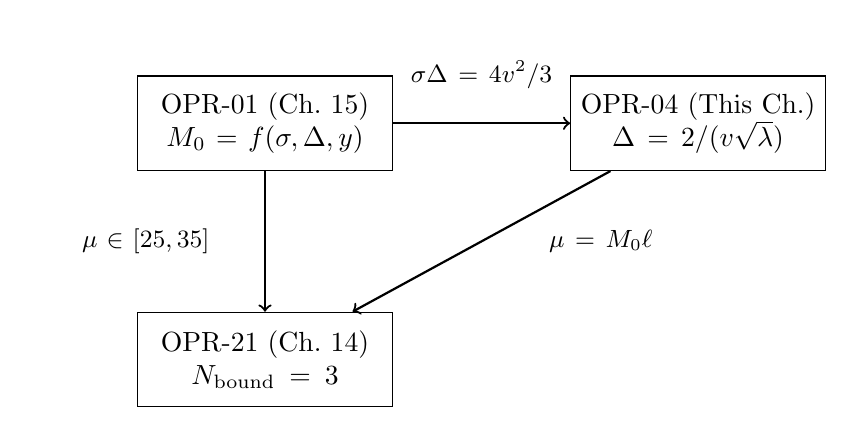
\begin{tikzpicture}[node distance=2.5cm, auto,
    every node/.style={rectangle, draw, minimum width=3cm, minimum height=1.2cm,
    align=center, text width=3cm}]

    \node (opr01) {OPR-01 (Ch.~15)\\$M_0 = f(\sigma,\Delta,y)$};
    \node (opr04) [right of=opr01, xshift=3cm] {OPR-04 (This Ch.)\\$\Delta = 2/(v\sqrt{\lambda})$};
    \node (opr21) [below of=opr01, yshift=-0.5cm] {OPR-21 (Ch.~14)\\$N_{\rm bound} = 3$};

    \draw[->, thick] (opr01) -- node[above, draw=none, text width=2.5cm, align=center]
        {\small $\sigma\Delta = 4v^2/3$} (opr04);
    \draw[->, thick] (opr04) -- node[right, draw=none, text width=2cm, align=center]
        {\small $\mu = M_0 \ell$} (opr21);
    \draw[->, thick] (opr01) -- node[left, draw=none, text width=2cm, align=center]
        {\small $\mu \in [25,35]$} (opr21);
\end{tikzpicture}
\end{center}

\textbf{Read next:}
\begin{itemize}[nosep]
    \item Chapter~15 (OPR-01): How $M_0$ emerges from $\sigma$ and $\Delta$
    \item Chapter~14 (OPR-21): How the $\mu$-window yields three generations
    \item Audit: \texttt{canon/opr/OPR\_REGISTRY.md} for full OPR status
\end{itemize}
\end{tcolorbox}

% ==============================================================================
% END OF CHAPTER
% ==============================================================================
